\documentclass[aspectratio=169]{beamer}

% ---------------------------------------------------------

\usepackage[utf8]{inputenc}
\usepackage[T1]{fontenc}
\usepackage[english]{babel}

% ---------------------------------------------------------

\usepackage{appendixnumberbeamer}

\setbeamertemplate{navigation symbols}{}

\addtobeamertemplate{footline}{%
	\hspace*{\fill}%
	\llap{%
		\insertframenumber\,/\,\inserttotalframenumber%
		\hspace{5pt}%
	}
	\vskip4pt%
}

% ---------------------------------------------------------

\usepackage{subcaption}

\usepackage{changepage}

\usepackage{tikz}

% ---------------------------------------------------------

\usepackage{amsmath}

\usepackage{mathtools}

\usepackage{mathpartir}
\let\TirName\textsc
\renewcommand{\DefTirName}[1]{\hypertarget{#1}{\TirName {#1}}}
\newcommand{\RefTirName}[1]{\hyperlink{#1}{\TirName {#1}}}

\let\oldexists\exists
\let\exists\relax\DeclareMathOperator{\exists}{\oldexists}
\let\oldforall\forall
\let\forall\relax\DeclareMathOperator{\forall}{\oldforall}

\DeclareMathOperator{\lambdaAbs}{\lambda}
\DeclareMathOperator{\muAbs}{\mu}
\DeclareMathOperator{\nuAbs}{\nu}

% ---------------------------------------------------------

\usepackage{overtools}

\usepackage{macros}

\usepackage{mylistings}

% ---------------------------------------------------------

\title{
	Tail Modulo Cons, \\
	\OCaml, \\
	and Relational Separation Logic
}
\author{
	\underline{Clément Allain} \\
	Frédéric Bour \\
	Basile Clément \\
	François Pottier \\
	Gabriel Scherer
}

% ---------------------------------------------------------
% ---------------------------------------------------------

\begin{document}

% ---------------------------------------------------------

\begin{frame}
\titlepage
\end{frame}

% ---------------------------------------------------------

\begin{frame}{Tail Modulo Cons, \OCaml, and Relational Separation Logic}
\begin{figure}
  \begin{subfigure}[b]{0.16\textwidth}
    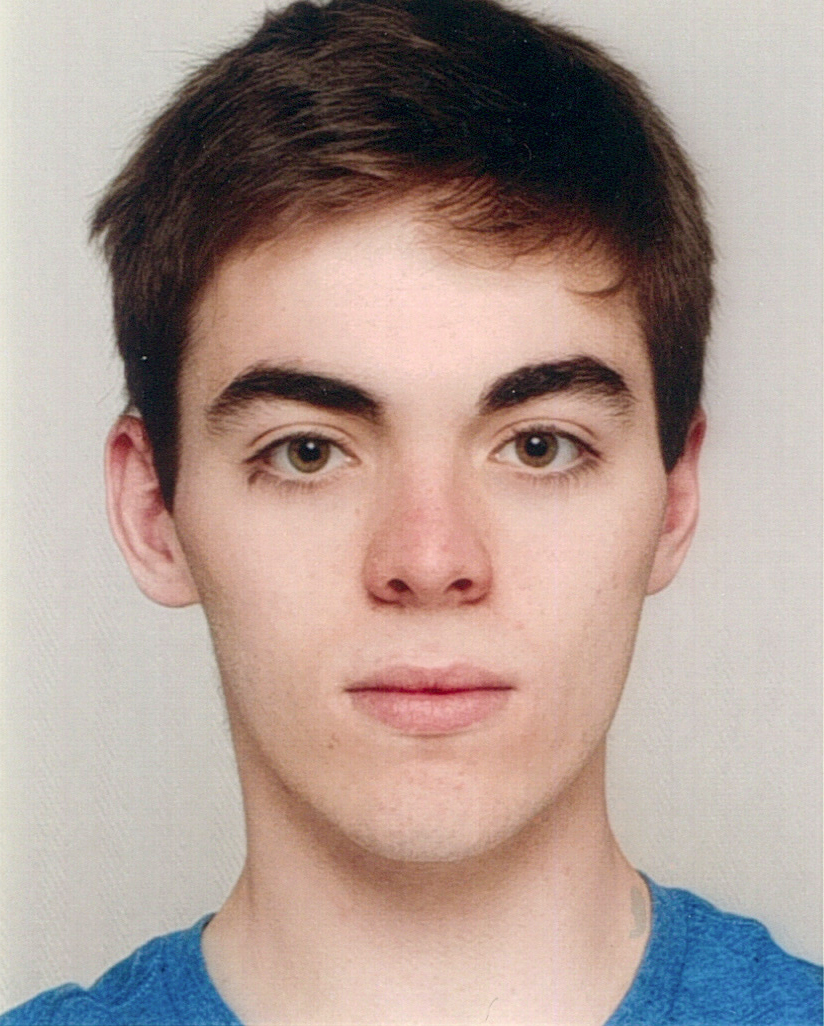
\includegraphics[scale=0.6]{images/clement_allain.jpg}
    \caption*{\footnotesize Clément \\ Allain}
  \end{subfigure}
  \begin{subfigure}[b]{0.16\textwidth}
    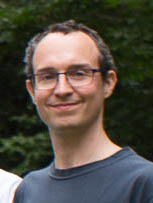
\includegraphics[scale=1.3]{images/frederic_bour.jpg}
    \caption*{\footnotesize Frédéric \\ Bour}
  \end{subfigure}
  \begin{subfigure}[b]{0.16\textwidth}
    
\includegraphics[scale=0.4]{images/basile_clement.jpg}
    \caption*{\footnotesize Basile \\ Clément}
  \end{subfigure}
  \begin{subfigure}[b]{0.16\textwidth}
    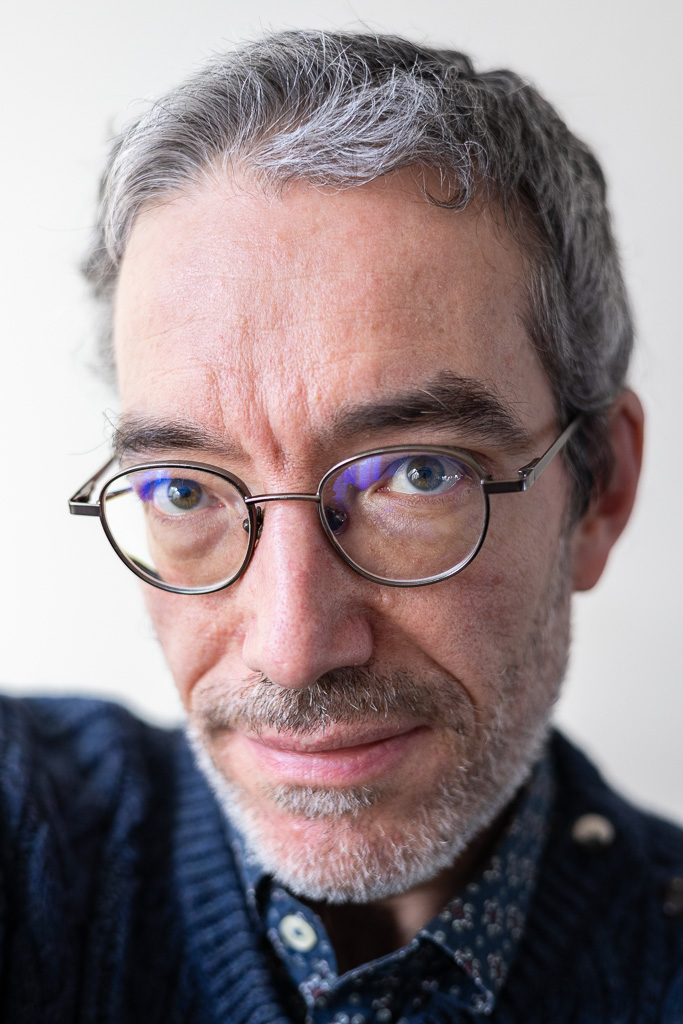
\includegraphics[scale=0.078]{images/francois_pottier.jpg}
    \caption*{\footnotesize François \\ Pottier}
  \end{subfigure}
  \begin{subfigure}[b]{0.16\textwidth}
    
\includegraphics[scale=1.2]{images/gabriel_scherer.jpg}
    \caption*{\footnotesize Gabriel \\ Scherer}
  \end{subfigure}
\end{figure}
\end{frame}
\begin{frame}[fragile]{\texttt{map}: natural implementation}
\begin{lstlisting}
let rec %\textcolor{red}{map}% f xs =
  match xs with
  | [] ->
      []
  | x :: xs ->
      let y = f x in
      %\textcolor{cyan}{y ::}% %\textcolor{red}{map}% f xs
\end{lstlisting}
\vfill
\begin{lstlisting}
# List.init 250_000 (fun _ -> ())
  |> map Fun.id
  |> ignore
  ;;
Stack overflow during evaluation (looping recursion?).
\end{lstlisting}
\end{frame}

\begin{frame}[fragile]{\texttt{map}: accumulator-passing style}
\begin{minipage}{0.5\linewidth}
\begin{lstlisting}
let rec %\textcolor{red}{map\_aps}% %\textcolor{cyan}{acc}% f xs =
  match xs with
  | [] ->
      List.rev acc
  | x :: xs ->
      let y = f x in
      %\textcolor{red}{map\_aps}% %\textcolor{cyan}{(y ::\ acc)}% f xs
\end{lstlisting}
\end{minipage}
\begin{minipage}{0.45\linewidth}
\begin{lstlisting}
let map xs =
  %\textcolor{red}{map\_aps}% [] f xs




%%
\end{lstlisting}
\end{minipage}
\vfill
\begin{lstlisting}
# List.init 250_000 (fun _ -> ())
  |> map Fun.id
  |> ignore
  ;;
- : unit = ()
\end{lstlisting}
\end{frame}

%\begin{frame}{\texttt{map}: accumulator-passing style}
%\centering
%\begin{tikzpicture}[yscale=-1]
%    \draw [fill=cyan, fill opacity=0.4, dashed] (0,0) rectangle (3,1) node [pos=.5] {\texttt{acc}} ;
%    \draw [fill=magenta, fill opacity=0.4] (4,0) rectangle (5,1) node [pos=.5] {\texttt{x}} ;
%    \draw [fill=magenta, fill opacity=0.4, dashed] (6,0) rectangle (9,1) node [pos=.5] {\texttt{xs}} ;
%    \draw [thick, ->] (5,0.5) -- (6,0.5) ;
%    
%    \draw [fill=cyan, fill opacity=0.4, dashed] (0,1.5) rectangle (3,2.5) node [pos=.5] {\texttt{acc}} ;
%    \draw [fill=cyan, fill opacity=0.4] (4,1.5) rectangle (5,2.5) node [pos=.5] {\texttt{f x}} ;
%    \draw [fill=magenta, fill opacity=0.4, dashed] (6,1.5) rectangle (9,2.5) node [pos=.5] {\texttt{xs}} ;
%    
%    \draw [fill=cyan, fill opacity=0.4, dashed] (0,3) rectangle (3,4) node [pos=.5] {\texttt{acc}} ;
%    \draw [fill=cyan, fill opacity=0.4] (4,3) rectangle (5,4) node [pos=.5] {\texttt{f x}} ;
%    \draw [fill=magenta, fill opacity=0.4, dashed] (6,3) rectangle (9,4) node [pos=.5] {\texttt{xs}} ;
%    \draw [thick, ->] (4,3.5) -- (3,3.5) ;
%\end{tikzpicture}
%\end{frame}
%
%\begin{frame}{\texttt{map}: can we do better?}
%\centering
%\begin{tikzpicture}[yscale=-1]
%    \draw [fill=cyan, fill opacity=0.4, dashed] (0,0) rectangle (3,1) node [pos=.5] {\texttt{acc}} ;
%    \draw [fill=magenta, fill opacity=0.4] (4,0) rectangle (5,1) node [pos=.5] {\texttt{x}} ;
%    \draw [fill=magenta, fill opacity=0.4, dashed] (6,0) rectangle (9,1) node [pos=.5] {\texttt{xs}} ;
%    \draw [thick, ->] (5,0.5) -- (6,0.5) ;
%    
%    \draw [fill=cyan, fill opacity=0.4, dashed] (0,1.5) rectangle (3,2.5) node [pos=.5] {\texttt{acc}} ;
%    \draw [fill=cyan, fill opacity=0.4] (4,1.5) rectangle (5,2.5) node [pos=.5] {\texttt{f x}} ;
%    \draw [fill=magenta, fill opacity=0.4, dashed] (6,1.5) rectangle (9,2.5) node [pos=.5] {\texttt{xs}} ;
%    
%    \draw [fill=cyan, fill opacity=0.4, dashed] (0,3) rectangle (3,4) node [pos=.5] {\texttt{acc}} ;
%    \draw [fill=cyan, fill opacity=0.4] (4,3) rectangle (5,4) node [pos=.5] {\texttt{f x}} ;
%    \draw [fill=magenta, fill opacity=0.4, dashed] (6,3) rectangle (9,4) node [pos=.5] {\texttt{xs}} ;
%    \draw [thick, ->] (3,3.5) -- (4,3.5) ;
%\end{tikzpicture}
%\end{frame}

\begin{frame}[fragile]{\texttt{map}: destination-passing style}
\begin{minipage}{0.5\linewidth}
\begin{lstlisting}
let rec %\textcolor{red}{map\_dps}% %\textcolor{cyan}{dst}% f xs =
  match xs with
  | [] ->
      %\textcolor{olive}{set\_field dst 1 []}%
  | x :: xs ->
      let y = f x in
      let dst' = y :: %\textcolor{olive}{\_}% in
      %\textcolor{olive}{set\_field dst 1 dst'}% ;
      %\textcolor{red}{map\_dps}% %\textcolor{cyan}{dst'}% f xs
\end{lstlisting}
\end{minipage}
\begin{minipage}{0.45\linewidth}
\begin{lstlisting}
let map f xs =
  match xs with
  | [] ->
      []
  | x :: xs ->
      let y = f x in
      let dst = y :: %\textcolor{olive}{\_}% in
      %\textcolor{red}{map\_dps}% dst f xs ;
      dst
\end{lstlisting}
\end{minipage}
\vfill
\begin{lstlisting}
# List.init 250_000 (fun _ -> ())
  |> map Fun.id
  |> ignore
  ;;
- : unit = ()
\end{lstlisting}
\end{frame}

\begin{frame}[fragile]{\texttt{map}: Tail Modulo Constructor (TMC)}
\begin{lstlisting}
let%\textcolor{olive}{[@tail\_mod\_cons]}% rec %\textcolor{red}{map}% f xs =
  match xs with
  | [] ->
      []
  | x :: xs ->
      let y = f x in
      %\textcolor{cyan}{y ::}% %\textcolor{red}{map}% f xs
\end{lstlisting}
\vfill
\begin{lstlisting}
# List.init 250_000 (fun _ -> ())
  |> map Fun.id
  |> ignore
  ;;
- : unit = ()
\end{lstlisting}
\end{frame}

\begin{frame}{TMC transformation}
\large
\begin{itemize}
  \setlength\itemsep{0.3em}
  \item \textbf{Safe:} performed by the \OCaml compiler.
  \item \textbf{Explicit:} \texttt{[@tail\_mod\_cons]} annotation.
  \setlength\itemsep{1.7em}
  \item \textbf{Generality:}
    \begin{itemize}
      \item Works on any algebraic data type (lists, trees, \etc).
      \item Supports mutually recursive functions.
    \end{itemize}
  \item \textbf{Implementation details:} see the paper.
  \setlength\itemsep{0.3em}
  \item \textbf{Performance:} see benchmarks in the paper.
  \item \textbf{Feature adoption:} see survey in the paper.
  \setlength\itemsep{1.7em}
  \item \textbf{Soundness:} formally verified in \Coq in an simplified setting \dots
\end{itemize}
\end{frame}
\begin{frame}{\DataLang: syntax}
\centering
\color{lightgray}
\begin{tabular}{lclcl}
    $\datalangIdx[]$
    & $\ni$ &
    $\datalangIdx$
    & $\Coloneqq$ &
    $\datalangZero \mid \datalangOne \mid \datalangTwo$
  \\
    $\datalangTag[]$
    & $\ni$ &
    $\datalangTag$
  \\
    $\datalangBool[]$
    & $\ni$ &
    $\datalangBool$
	\\
		$\datalangLoc[]$
		& $\ni$ &
		$\datalangLoc$
  \\
    $\datalangFn[]$
    & $\ni$ &
    $\datalangFn$
  \\
    $\datalangVar[]$
    & $\ni$ &
    $\datalangVar, \datalangVarTwo$
	\\
    $\datalangVal[]$
    & $\ni$ &
    $\datalangVal, \datalangValTwo$
    & $\Coloneqq$ &
    $\datalangUnit \mid \datalangIdx \mid \datalangTag \mid \datalangBool \mid \datalangLoc \mid \mathcolor{red}{\datalangFnptr{\datalangFn}}$
  \\
    $\datalangExpr[]$
    & $\ni$ &
    $\datalangExpr$
    & $\Coloneqq$ &
    $\datalangVal \mid \datalangVar \mid \datalangLet{\datalangVar}{\datalangExpr_1}{\datalangExpr_2} \mid \datalangCall{\datalangExpr_1}{\overline{\datalangExpr_2}}$
  \\
    &&
    & | &
    $\datalangEq{\datalangExpr_1}{\datalangExpr_2} \mid \datalangIf{\datalangExpr_0}{\datalangExpr_1}{\datalangExpr_2}$
  \\
    &&
    & | &
    $\mathcolor{orange}{\datalangBlock{\datalangTag}{\datalangExpr_1}{\datalangExpr_2}}$
  \\
    &&
    & | &
    $\datalangLoad{\datalangExpr_1}{\datalangExpr_2} \mid \datalangStore{\datalangExpr_1}{\datalangExpr_2}{\datalangExpr_3}$
  \\
    $\datalangDef[]$
    & $\ni$ &
    $\datalangDef$
    & $\Coloneqq$ &
    $\mathcolor{violet}{\datalangRec{\overline{\datalangVar}}{\datalangExpr}}$
  \\
    $\datalangProg[]$
    & $\ni$ &
    $\datalangProg$
    & $\coloneqq$ &
    $\mathcolor{blue}{\datalangFn[] \finmap \datalangDef[]}$
  \\
    $\datalangState[]$
    & $\ni$ &
    $\datalangState$
    & $\coloneqq$ &
    $\datalangLoc[] \finmap \datalangVal[]$
  \\
    $\datalangConfig[]$
    & $\ni$ &
    $\datalangConfig$
    & $\coloneqq$ &
    $\datalangExpr[] \times \datalangState[]$
\end{tabular}
\vfill
\end{frame}

\begin{frame}[fragile]{\DataLang: \texttt{map}}
\begin{lstlisting}[basicstyle=\ttfamily\Large]
%\textcolor{red}{map}% |-> fun f xs ->
  match xs with
  | [] ->
      []
  | x :: xs ->
      let y = f x in
      y :: @%\textcolor{red}{map}% f xs
\end{lstlisting}
\end{frame}

\begin{frame}[fragile]{\DataLang: \texttt{map} (transformed)}
\begin{minipage}{.5\columnwidth}
\begin{lstlisting}
%\textcolor{red}{map\_dps}% |-> fun dst idx f xs ->
  match xs with
  | [] ->
      dst.(idx) <- []
  | x :: xs ->
      let y = f x in
      let dst' = y :: ?? in
      dst.(idx) <- dst' ;
      @%\textcolor{red}{map\_dps}% dst' 2 f xs
\end{lstlisting}
\end{minipage}
\begin{minipage}{.49\columnwidth}
\begin{lstlisting}
map_dir |-> fun f xs ->
  match xs with
  | [] ->
      []
  | x :: xs ->
      let y = f x in
      let dst = y :: ?? in
      @%\textcolor{red}{map\_dps}% dst 2 f xs ;
      dst
\end{lstlisting}
\end{minipage}
\end{frame}

\begin{frame}{TMC transformation}
\LARGE
\begin{mathpar}
    \datalangExpr_s \tmcDir{\datalangRenaming} \datalangExpr_t
  \and
    \datalangDef_s \tmcDir{\datalangRenaming} \datalangDef_t
  \\\\
    (\datalangExpr_\mathit{dst}, \datalangExpr_\mathit{idx}, \datalangExpr_s) \tmcDps{\datalangRenaming} \datalangExpr_t
  \and
    \datalangDef_s \tmcDps{\datalangRenaming} \datalangDef_t
  \\\\
    \datalangProg_s \tmc \datalangProg_t
\end{mathpar}
\end{frame}

\begin{frame}{Transformation soundness}
\large
\centering
\begin{tabular}{ccc}
    $\datalangProg_s \tmc \datalangProg_t$
    &&
    program $\datalangProg_s$ transforms into program $\datalangProg_t$
  \\\\
  \onslide<4->{
    $\Downarrow$
  \\\\
    $\datalangProg_s \iSimSymbol \datalangProg_t$
    &&
    program $\datalangProg_t$ simulates program $\datalangProg_s$
  \\
    &&
    (\emph{relational separation logic}, \Simuliris)
  }
  \\\\
    $\Downarrow$
  \\\\
    $\datalangProg_s \refined \datalangProg_t$
    &&
    program $\datalangProg_t$ refines program $\datalangProg_s$
  \\
    &&
    (termination-preserving refinement)
\end{tabular}
\begin{overbox}<2>
  \centering
  \textbf{Termination-preserving behavioral refinement} \\
  \bigskip
  \begin{tabular}{rcl}
      $\datalangProg_s \mathcolor{magenta}{\refined} \datalangProg_t$
      & $\coloneqq$ &
      $\forall \datalangFn \in \dom{\datalangProg_s}, \datalangVal_s, \datalangVal_t \ldotp$
    \\
      &&
      $\wf{\datalangVal_s} \wedge \datalangVal_s \similar \datalangVal_t \implies$
    \\
      &&
      $\datalangCall{\datalangFnptr{\datalangFn}}{\datalangVal_s} \mathcolor{orange}{\refined} \datalangCall{\datalangFnptr{\datalangFn}}{\datalangVal_t}$
    \\\\
      $\datalangExpr_s \mathcolor{orange}{\refined} \datalangExpr_t$
      & $\coloneqq$ &
      $\forall b_t \in \mathcolor{cyan}{\mathrm{behaviours}}_{\datalangProg_t} (\datalangExpr_t) \ldotp$
    \\
      &&
      $\exists b_s \in \mathcolor{cyan}{\mathrm{behaviours}}_{\datalangProg_s} (\datalangExpr_s) \ldotp
          b_s \mathcolor{blue}{\refined} b_t$
    \\\\
      $\mathcolor{cyan}{\mathrm{behaviours}}_{\datalangProg} (\datalangExpr)$
      & $\coloneqq$ &
      $\{ \constr[\datalangExpr']{Conv} \mid \dots \} \uplus \{ \constr{Div} \mid \diverges{\datalangProg}{(\datalangExpr, \emptyset)} \}$
  \end{tabular}
\end{overbox}
\begin{overbox}<5>
  \centering
  \textbf{Relational separation logic}
  \begin{mathpar}
    \inferrule*[lab=rel-pure]
      {
        \mathcolor{blue}{\datalangExpr_s} \pureStep{\mathcolor{blue}{p_s}} \mathcolor{blue}{\datalangExpr_s'}
      \and
        \mathcolor{magenta}{\datalangExpr_t} \pureStep{\mathcolor{magenta}{p_t}}\mathcolor{magenta}{\datalangExpr_t'}
      \and
        \iSim{
          \iPred
        }{
          \mathcolor{blue}{\datalangExpr_s'}
        }{
          \mathcolor{magenta}{\datalangExpr_t'}
        }
      }{
        \iSim{
          \iPred
        }{
          \mathcolor{blue}{\datalangExpr_s}
        }{
          \mathcolor{magenta}{\datalangExpr_t}
        }
      }
    \\
    \inferrule*[lab=rel-source-load]
      {
        (\mathcolor{blue}{\datalangLoc} + \mathcolor{blue}{\datalangIdx}) \iPointsto_s \mathcolor{blue}{\datalangVal_s}
      \and
        (\mathcolor{blue}{\datalangLoc} + \mathcolor{blue}{\datalangIdx}) \iPointsto_s \mathcolor{blue}{\datalangVal_s} \iWand
        \iSim{\iPred}{\mathcolor{blue}{\datalangVal_s}}{\mathcolor{magenta}{\datalangExpr_t}}
      }{
        \iSim{\iPred}{\datalangLoad{\mathcolor{blue}{\datalangLoc}}{\mathcolor{blue}{\datalangIdx}}}{\mathcolor{magenta}{\datalangExpr_t}}
      }
    \\
    \inferrule*[lab=rel-target-load]
      {
        (\mathcolor{magenta}{\datalangLoc} + \mathcolor{magenta}{\datalangIdx}) \iPointsto_t \mathcolor{magenta}{\datalangVal_t}
      \and
        (\mathcolor{magenta}{\datalangLoc} + \mathcolor{magenta}{\datalangIdx}) \iPointsto_t \mathcolor{magenta}{\datalangVal_t} \iWand
        \iSim{\iPred}{\mathcolor{blue}{\datalangExpr_s}}{\mathcolor{magenta}{\datalangVal_t}}
      }{
        \iSim{\iPred}{\mathcolor{blue}{\datalangExpr_s}}{\datalangLoad{\mathcolor{magenta}{\datalangLoc}}{\mathcolor{magenta}{\datalangIdx}}}
      }
  \end{mathpar}
\end{overbox}
\begin{overbox}<6>
  \centering
  \textbf{Abstract protocols \\ (calling conventions)}
  \medskip
  \begin{mathpar}
    \inferrule*[lab=rel-protocol]
      {
        \mathcolor{red}{\iProt} (\datalangExpr_s, \datalangExpr_t, \mathcolor{brown}{\iPredTwo})
      \and
        \forall \datalangExpr_s', \datalangExpr_t' \ldotp
        \mathcolor{brown}{\iPredTwo} (\datalangExpr_s', \datalangExpr_t') \iWand
        \iSim[
          \mathcolor{red}{\iProt}
        ]{
          \iPred
        }{
          \datalangExpr_s'
        }{
          \datalangExpr_t'
        }
      }{
        \iSim[
          \mathcolor{red}{\iProt}
        ]{
          \iPred
        }{
          \datalangExpr_s
        }{
          \datalangExpr_t
        }
      }
  \end{mathpar}
\end{overbox}
\only<7>{}
\end{frame}

\begin{frame}{Specification in separation logic}
\LARGE
\[
  \iSimvHoarePretty{
    ???
  }{
    \datalangCall{\datalangFnptr{\texttt{map}}}{\mathcolor{magenta}{\datalangVal_s}}
  }{
    \datalangCall{\datalangFnptr{\texttt{map\_dir}}}{\mathcolor{magenta}{\datalangVal_t}}
  }{
    ???
  }
\]
\vfill
\[
  \iSimvHoarePretty{
    ???
  }{
    \datalangCall{\datalangFnptr{\texttt{map}}}{\mathcolor{magenta}{\datalangVal_s}}
  }{
    \datalangCall{\datalangFnptr{\texttt{map\_dps}}}{\mathcolor{blue}{\datalangLoc}\ \datalangIdx\ \mathcolor{magenta}{\datalangVal_t}}
  }{
    ???
  }
\]
\end{frame}

\begin{frame}{Direct transformation}
\Large
\[
  \iSimvHoarePretty{
    \mathcolor{magenta}{\datalangVal_s} \iSimilar \mathcolor{magenta}{\datalangVal_t}
  }{
    \datalangCall{\datalangFnptr{\texttt{map}}}{\mathcolor{magenta}{\datalangVal_s}}
  }{
    \datalangCall{\datalangFnptr{\texttt{map\_dir}}}{\mathcolor{magenta}{\datalangVal_t}}
  }{
    \mathcolor{cyan}{\datalangValTwo_s}, \mathcolor{cyan}{\datalangValTwo_t} \ldotp
    \mathcolor{cyan}{\datalangValTwo_s} \iSimilar \mathcolor{cyan}{\datalangValTwo_t}
  }
\]
\vfill
\begin{mathpar}
  \inferrule*[lab=rel-dir (\Simuliris)]
    {
      \datalangFn \in \dom{\datalangProg_s}
    \\\\
      \mathcolor{magenta}{\datalangVal_s} \iSimilar \mathcolor{magenta}{\datalangVal_t}
    \\\\
      \forall \mathcolor{cyan}{\datalangValTwo_s}, \mathcolor{cyan}{\datalangValTwo_t} \ldotp
      \mathcolor{cyan}{\datalangValTwo_s} \iSimilar \mathcolor{cyan}{\datalangValTwo_t} \iWand
      \iPred (\mathcolor{cyan}{\datalangValTwo_s}, \mathcolor{cyan}{\datalangValTwo_t})
    }{
      \iSim{
        \iPred
      }{
        \datalangCall{\datalangFnptr{\datalangFn}}{\mathcolor{magenta}{\datalangVal_s}}
      }{
        \datalangCall{\datalangFnptr{\datalangFn}}{\mathcolor{magenta}{\datalangVal_t}}
      }
    }
\end{mathpar}
\end{frame}

\begin{frame}{DPS transformation}
\large
\[
  \iSimvHoarePretty{
    \mathcolor{magenta}{\datalangVal_s} \iSimilar \mathcolor{magenta}{\datalangVal_t} \iSep
    (\mathcolor{blue}{\datalangLoc} + \datalangIdx) \iPointsto_t \datalangHole
  }{
    \datalangCall{\datalangFnptr{\texttt{map}}}{\mathcolor{magenta}{\datalangVal_s}}
  }{
    \datalangCall{\datalangFnptr{\texttt{map\_dps}}}{\mathcolor{blue}{\datalangLoc}\ \datalangIdx\ \mathcolor{magenta}{\datalangVal_t}}
  }{
    \mathcolor{cyan}{\datalangValTwo_s}, \datalangUnit \ldotp
      \exists \mathcolor{cyan}{\datalangValTwo_t} \ldotp
      \mathcolor{cyan}{\datalangValTwo_s} \iSimilar \mathcolor{cyan}{\datalangValTwo_t} \iSep
      (\mathcolor{blue}{\datalangLoc} + \datalangIdx) \iPointsto_t \mathcolor{cyan}{\datalangValTwo_t}
  }
\]
\vfill
\begin{mathpar}
  \inferrule*[lab=rel-dps]
    {
      \datalangRenaming [\datalangFn] = \datalangFn_\mathit{dps}
    \\\\
      \mathcolor{magenta}{\overline{\datalangVal_s}} \iSimilar \mathcolor{magenta}{\overline{\datalangVal_t}}
    \\\\
      \mathcolor{blue}{\datalangLoc} \iPointsto_t \overline{\datalangVal}
    \\\\
      \forall \mathcolor{cyan}{\datalangValTwo_s}, \mathcolor{cyan}{\datalangValTwo_t} \ldotp
      \mathcolor{cyan}{\datalangValTwo_s} \iSimilar \mathcolor{cyan}{\datalangValTwo_t} \iWand
      \mathcolor{blue}{\datalangLoc} \iPointsto_t \overline{\datalangVal} [\datalangIdx \mapsto \mathcolor{cyan}{\datalangValTwo_t}] \iWand
      \iPred (\mathcolor{cyan}{\datalangValTwo_s}, \datalangUnit)
    }{
      \iSim{
        \iPred
      }{
        \datalangCall{\datalangFnptr{\datalangFn}}{\mathcolor{magenta}{\overline{\datalangVal_s}}}
      }{
        \datalangCall{\datalangFnptr{\datalangFn_\mathit{dps}}}{\mathcolor{blue}{\datalangLoc} \ \datalangIdx\ \mathcolor{magenta}{\overline{\datalangVal_t}}}
      }
    }
  \\
  \inferrule*[lab=rel-protocol]
    {
      \mathcolor{red}{\iProt} (\datalangExpr_s, \datalangExpr_t, \mathcolor{brown}{\iPredTwo})
    \and
      \forall \datalangExpr_s', \datalangExpr_t' \ldotp
      \mathcolor{brown}{\iPredTwo} (\datalangExpr_s', \datalangExpr_t') \iWand
      \iSim[
        \mathcolor{red}{\iProt}
      ]{
        \iPred
      }{
        \datalangExpr_s'
      }{
        \datalangExpr_t'
      }
    }{
      \iSim[
        \mathcolor{red}{\iProt}
      ]{
        \iPred
      }{
        \datalangExpr_s
      }{
        \datalangExpr_t
      }
    }
\end{mathpar}
\end{frame}

\begin{frame}{Conclusion}
\Large
\begin{itemize}
  \setlength\itemsep{1.5em}
  \item Implementation of the TMC transformation in the \OCaml compiler.
  \item Mechanized soundness proof using \emph{relational separation logic}.
  \item \emph{Abstract protocols} to support different calling conventions: APS, inlining.
\end{itemize}
\end{frame}


% ---------------------------------------------------------

\begin{frame}[plain, noframenumbering]
\LARGE
\begin{center}
	Thank you for your attention!
\end{center}
\end{frame}

% ---------------------------------------------------------

\appendix
\begin{frame}{Simulation}
\scriptsize
\begin{align*}
		\mathrm{sim \mathhyphen body}_\iProt
		&\coloneqq
		\begin{array}{l}
				\lambdaAbs \textcolor{\iSimGfpColor}{sim} \ldotp
				\lambdaAbs \textcolor{\iSimLfpColor}{sim \mathhyphen inner} \ldotp
				\lambdaAbs {(\iPred, \datalangExpr_s, \datalangExpr_t)} \ldotp
				\forall \datalangState_s, \datalangState_s \ldotp
				\mathrm{I} (\datalangState_s, \datalangState_t)
				\iWand \iBupd
			\\
				\bigvee \left[ \begin{array}{ll}
							\circled{1}
						&
							\mathrm{I} (\datalangState_s, \datalangState_t) \iSep
							\iPred (\datalangExpr_s, \datalangExpr_t)
					\\
					        \circled{2}
                        &
                            \mathrm{I} (\datalangState_s, \datalangState_t) \iSep
							\mathrm{strongly \mathhyphen stuck}_{\datalangProg_s} (\datalangExpr_s) \iSep
							\mathrm{strongly \mathhyphen stuck}_{\datalangProg_t} (\datalangExpr_s)
					\\
							\circled{3}
						&
							\exists \datalangExpr_s', \datalangState_s' \ldotp
							(\datalangExpr_s, \datalangState_s) \step{\datalangProg_s}^+ (\datalangExpr_s', \datalangState_s') \iSep
							\mathrm{I} (\datalangState_s', \datalangState_t) \iSep
							\textcolor{\iSimLfpColor}{sim \mathhyphen inner} (\iPred, \datalangExpr_s', \datalangExpr_t)
					\\
							\circled{4}
						&
						\mathrm{reducible}_{\datalangProg_t} (\datalangExpr_t, \datalangState_t) \iSep
						\forall \datalangExpr_t', \datalangState_t' \ldotp
						(\datalangExpr_t, \datalangState_t) \step{\datalangProg_t} (\datalangExpr_t', \datalangState_t')
						\iWand \iBupd
				\\
                        &
						\bigvee \left[ \begin{array}{ll}
									\circled{A}
								&
									\mathrm{I} (\datalangState_s, \datalangState_t') \iSep
									\textcolor{\iSimLfpColor}{sim \mathhyphen inner} (\iPred, \datalangExpr_s, \datalangExpr_t')
							\\
									\circled{B}
								&
									\exists \datalangExpr_s', \datalangState_s' \ldotp
									(\datalangExpr_s, \datalangState_s) \step{\datalangProg_s}^+ (\datalangExpr_s', \datalangState_s') \iSep
									\mathrm{I} (\datalangState_s', \datalangState_t') \iSep
									\textcolor{\iSimGfpColor}{sim} (\iPred, \datalangExpr_s', \datalangExpr_t')
						\end{array} \right.
					\\
							\circled{5}
						&
							\exists \datalangEctx_s, \datalangExpr_s', \datalangEctx_t, \datalangExpr_t', \iPredTwo \ldotp
					\\
					    &
					        \datalangExpr_s = \datalangEctx_s [\datalangExpr_s'] \iSep
							\datalangExpr_t = \datalangEctx_t [\datalangExpr_t'] \iSep
						    \iProt (\iPredTwo, \datalangExpr_s', \datalangExpr_t') \iSep
						    \mathrm{I} (\datalangState_s, \datalangState_t) \iSep {}
					\\
                        &
						\forall \datalangExpr_s'', \datalangExpr_t'' \ldotp
						\iPredTwo (\datalangExpr_s'', \datalangExpr_t'') \iWand
						\textcolor{\iSimLfpColor}{sim \mathhyphen inner} (\iPred, \datalangEctx_s [\datalangExpr_s''], \datalangEctx_t [\datalangExpr_t''])
				\end{array} \right.
		\end{array}
	\\
	    \mathrm{\color{\iSimLfpColor}{sim \mathhyphen inner}}_\iProt
	    &\coloneqq
	    \lambdaAbs \textcolor{\iSimGfpColor}{sim} \ldotp
	    \muAbs \textcolor{\iSimLfpColor}{sim \mathhyphen inner} \ldotp
	    \mathrm{sim \mathhyphen body}_\iProt (sim, \textcolor{\iSimLfpColor}{sim \mathhyphen inner})
	\\
		\mathrm{\color{\iSimGfpColor}{sim}}_\iProt
		&\coloneqq
		\nuAbs \textcolor{\iSimGfpColor}{sim} \ldotp
		\mathrm{\color{\iSimLfpColor}{sim \mathhyphen inner}}_\iProt (\textcolor{\iSimGfpColor}{sim})
	\\
		\iSim[\iProt]{\iPred}{\datalangExpr_s}{\datalangExpr_t}
		&\coloneqq
		\mathrm{\color{\iSimGfpColor}{sim}}_\iProt (\iPred, \datalangExpr_s, \datalangExpr_t)
	\\
	   \iSimv[\iProt]{\iPred}{\datalangExpr_s}{\datalangExpr_t}
	   &\coloneqq
	   \iSim[\iProt]{\lambdaAbs (\datalangExpr_s', \datalangExpr_t') \ldotp \exists \datalangVal_s, \datalangVal_t \ldotp \datalangExpr_s' = \datalangVal_s \iSep \datalangExpr_t' = \datalangVal_t \iSep \iPred (\datalangVal_s, \datalangVal_t)}{\datalangExpr_s}{\datalangExpr_t}
\end{align*}
\end{frame}

\begin{frame}{Admissibility}
\large
\[
  \iPersistent \left(
    \forall \iPredTwo, \datalangExpr_s, \datalangExpr_t \ldotp
    \iProt (\iPredTwo, \datalangExpr_s, \datalangExpr_t) \iWand
    \mathrm{sim \mathhyphen inner}_\bot (\lambdaAbs (\_, \datalangExpr_s', \datalangExpr_t') \ldotp \iSim[\iProt]{\iPredTwo}{\datalangExpr_s'}{\datalangExpr_t'}) (\bot, \datalangExpr_s, \datalangExpr_t)
  \right)
\]
\vfill
\[
  \Admissible{\iProt} \iWand
  \iSim[\iProt]{\iPred}{\datalangExpr_s}{\datalangExpr_t} \iWand
  \iSim[\bot]{\iPred}{\datalangExpr_s}{\datalangExpr_t}
\]
\end{frame}

\begin{frame}{TMC protocol}
\begin{tabular}{rcl}
        $\iProt_\mathrm{dir} (\iPredTwo, \datalangExpr_s, \datalangExpr_t)$
        & $\coloneqq$ &
        $\exists \datalangFn, \datalangVal_s, \datalangVal_t \ldotp$
    \\
        &&
        $\datalangFn \in \dom{\datalangProg_s} \iSep {}$
    \\
        &&
        $\datalangExpr_s = \datalangCall{\datalangFnptr{\datalangFn}}{\datalangVal_s} \iSep
        \datalangExpr_t = \datalangCall{\datalangFnptr{\datalangFn}}{\datalangVal_t} \iSep
        \datalangVal_s \iSimilar \datalangVal_t \iSep {}$
    \\
        &&
        $\forall \datalangVal_s', \datalangVal_t' \ldotp
        \datalangVal_s' \iSimilar \datalangVal_t' \iWand
        \iPredTwo (\datalangVal_s', \datalangVal_t')$
    \\\\
        $\iProt_\mathrm{DPS} (\iPredTwo, \datalangExpr_s, \datalangExpr_t)$
        & $\coloneqq$ &
        $\exists \datalangFn, \datalangFn_\mathit{dps}, \datalangVal_s, \datalangLoc, \datalangIdx, \datalangVal_t \ldotp$
    \\
        &&
        $\datalangFn \in \dom{\datalangProg_s} \iSep
        \datalangRenaming [\datalangFn] = \datalangFn_\mathit{dps} \iSep {}$
    \\
        &&
        $\datalangExpr_s = \datalangCall{\datalangFnptr{\datalangFn}}{\datalangVal_s} \iSep
        \datalangExpr_t = \datalangCall{\datalangFnptr{\datalangFn_\mathit{dps}}}{\datalangPair{\datalangPair{\datalangLoc}{\datalangIdx}}{\datalangVal_t}} \iSep
        \datalangVal_s \iSimilar \datalangVal_t \iSep {}$
    \\
        &&
        $(\datalangLoc + \datalangIdx) \iPointsto \datalangHole \iSep {}$
    \\
        &&
        $\forall \datalangVal_s', \datalangVal_t' \ldotp
        (\datalangLoc + \datalangIdx) \iPointsto \datalangVal_t' \iSep
        \datalangVal_s' \iSimilar \datalangVal_t' \iWand
        \iPredTwo (\datalangVal_s', \datalangUnit)$
    \\\\
        $\iProt_\mathrm{TMC}$
        & $\coloneqq$ &
        $\iProt_\mathrm{dir} \sqcup \iProt_\mathrm{DPS}$
\end{tabular}
\end{frame}


% ---------------------------------------------------------

\end{document}
